\chapter{Useful formulas}
\begin{weekintro}
  You can expect that this page (or similar) will be provided to you in every midterm/final exam. For quizzes, a subset of the formulas may be provided as well.
\end{weekintro}

\begin{multicols}{2}

Laplace transform: $\laplace\braced*{f(t)} = \int_0^{\infty} e^{-st}
f(t)dt (=F(s))$

\vspace{0.5em}\hrule\vspace{0.5em}

\textbf{Properties}

Assuming \(\laplace\braced*{f(t)} = F(s)\), \quad \( \laplace\braced*{g(t)} = G(s)\):

\begin{itemize}
\item Linearity: \\$\laplace\braced*{c_1f(t)+c_2g(t)} = c_1F(s)+c_2G(s)$

\item Derivative in \(t\):
  \begin{align*}
    \laplace\braced*{f'(t)} &= sF(s)-f(0), \\
    \laplace\braced*{f''(t)} &= s^2F(s) - sf(0) - f'(0)
  \end{align*}

\item Integral in \(t\):
  \[\laplace\braced*{\int_{0}^{t}f(\tau) d\tau} = \frac{1}{s}F(s), \]

\item \(t\)-shift: $\laplace\braced*{\hstep(t-a)f(t-a)} = e^{-sa}F(s)$

  \vspace{0.5em}\hrule\vspace{0.5em}

\item \(s\)-shift:  $\laplace\braced*{e^{at}f(t)} = F(s-a)$
\item \(s\)-derivative:\\ $\laplace\braced*{tf(t)} = -F'(s)$, \quad $\laplace\braced*{t^nf(t)} = (-1)^n F^{(n)}(s)$
\item \(s\)-integral: $\laplace\braced*{\frac{f(t)}{t}} = \int_s^{\infty} F(\sigma) d\sigma$

  \vspace{0.5em}\hrule\vspace{0.5em}

\item Convolution: \\ $\laplace\braced*{(f*g)(t)} = F(s)G(s)$,
  \\where \((f * g)(t) = \int_{0}^{t}f(t-\tau)g(\tau)d\tau\)

\end{itemize}
\everymath{\displaystyle}
  \begin{center}
\rowcolors{1}{white}{gray!15}
\renewcommand{\arraystretch}{2}
\begin{tabular}{ |>{\centering\arraybackslash}m{1in}|>{\centering\arraybackslash}m{1in}|}
$f(t)$ & $F(s) = \laplace\braced*{f(t)}$\\\hline
$1$ & $\frac{1}{s}$ \\
$t^n$ & $\frac{n!}{s^{n+1}}$ \\
$e^{at}$ & $\frac{1}{s-a}$ \\
$\sin(\omega t)$ & $\frac{\omega}{s^2+\omega^2}$ \\
$\cos(\omega t)$ & $\frac{s}{s^2+\omega^2}$ \\
$e^{at}\sin(\omega t)$ & $\frac{\omega}{(s-a)^2+\omega^2}$ \\
$e^{at}\cos(\omega t)$ & $\frac{s-a}{(s-a)^2+\omega^2}$ \\
$\cosh(at)$ & $\frac{s}{s^2-a^2}$ \\
$\sinh(at)$ & $\frac{a}{s^2-a^2}$ \\
\end{tabular}
\end{center}

\end{multicols}

\vfill

\begin{minipage}{0.23\linewidth}
\(
\begin{vmatrix}
  A & B \\ C & D
\end{vmatrix} = AD - BC \)
\end{minipage}\hfill\begin{minipage}{0.23\linewidth}
  \centering
  \textbf{Rule of Sarrus}

  \vspace{1em}

  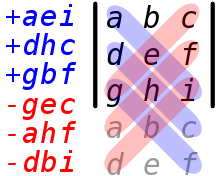
\includegraphics[width=.8\linewidth]{figs/rule-of-sarrus.png}
\end{minipage}\hfill\begin{minipage}{0.23\linewidth}
    \centering
    \textbf{Quadratic formula}

    \vspace{1em}
    Roots of \(ax^{2} + bx + c\) are

    \(x_{1,2} = \frac{-b \pm \sqrt{b^{2} - 4ac}}{2a}\)
  \end{minipage}\hfill\begin{minipage}{0.23\linewidth}
    \centering
 \textbf{Wronskian}

\vspace{1em}

\(W(x) = \begin{vmatrix}
    y_{1}(x) & y_{2}(x) \\
    y_{1}'(x) & y_{2}'(x)
  \end{vmatrix}\)

\end{minipage}

\vfill

\begin{minipage}{0.5\linewidth}
\begin{center}
\textbf{Variation of Parameters for 2nd order \ode{}s}

\vspace{1em}

\(y(x) = u_{1}(x) y_{1}(x) + u_{2}(x) y_{2}(x)\)

\(u_{1}'(x) = \frac{
  \begin{vmatrix}
    0 & y_{2}(x) \\
    f(x) & y_{2}'(x)
  \end{vmatrix}
}{  \begin{vmatrix}
    y_{1}(x) & y_{2}(x) \\
    y_{1}'(x) & y_{2}'(x)
  \end{vmatrix}
}\) \hfill \(u_{2}'(x) = \frac{
  \begin{vmatrix}
    y_{1}(x) & 0 \\
    y_{1}'(x) & f(x)
  \end{vmatrix}
}{  \begin{vmatrix}
    y_{1}(x) & y_{2}(x) \\
    y_{1}'(x) & y_{2}'(x)
  \end{vmatrix}
}\)
\end{center}
\end{minipage}\hfill\begin{minipage}{0.28\linewidth}
\begin{center}
\textbf{Trig. and hyperbolic trig. functions}

\vspace{1em}

  \begin{align*}
    \cos(x) = \frac{1}{2}e^{i x} + \frac{1}{2}e^{-i x} &\quad
    \sin(x) = \frac{1}{2i}e^{i x} - \frac{1}{2i}e^{-i x} \\
    \cosh(x) = \frac{1}{2}e^{x} + \frac{1}{2}e^{-x} &\quad
    \sinh(x) = \frac{1}{2}e^{x} - \frac{1}{2}e^{-x}
  \end{align*}
\end{center}

\end{minipage}


%%% Local Variables:
%%% mode: latex
%%% TeX-master: "main"
%%% End: